%----------------------------------------------------------------------
%----------------------------------------------------------------------
\section{Success Stories}

\begin{frame}[c]{Large-scale meta-learning for hyperparameter optimization}

\begin{itemize}
    \item Facebook has an internal self-service machine learning system
    \item Non-ML departments can integrate highly optimized machine learning models into their workflow
    \item Hyperparameters of the ML models are optimized with Bayesian optimization
    \item Training data for the models changes over time \item Hyperparameters are constantly re-optimized using meta-learning Bayesian optimization as described in \lit{\href{https://arxiv.org/abs/1802.02219}{Feurer et al. 2018}}
    \begin{figure}
        \centering
        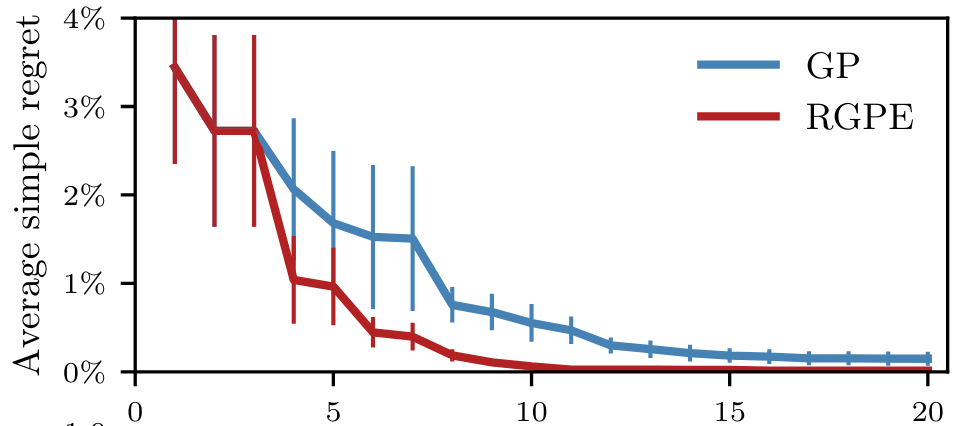
\includegraphics[width=0.5\textwidth]{images/success_stories/FB_RGPE.png}
        \caption{Bayesian optimization with meta-learning (RGPE) vs. vanilla Bayesian optimization (GP)}
    \end{figure}
\end{itemize}

\end{frame}

%-----------------------------------------------------------------------

\begin{frame}[c]{Auto-sklearn}
Extension of Auto-WEKA with focus on speed improvements and robustness:
\begin{figure}
    \centering
    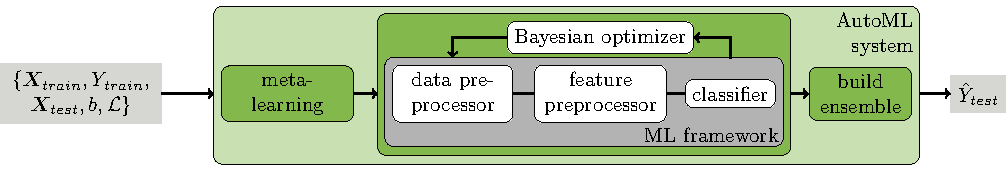
\includegraphics[width=0.9\textwidth]{images/success_stories/automlworkflow.pdf}
\end{figure}
\begin{itemize}
    \item Uses Meta-learning to warmstart Bayesian optimization
    \item Won the 1st AutoML challenge
    \item Open source (BSD) and trivial to use:
\end{itemize}
\begin{figure}
    \centering
    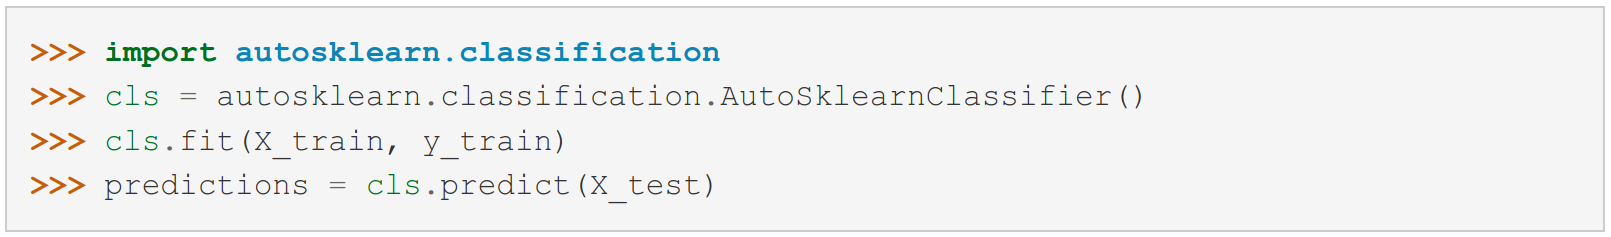
\includegraphics[width=0.9\textwidth]{images/success_stories/Auto-sklearn_01.png}
\end{figure}
Available at \href{automl.github.io/auto-sklearn}{automl.github.io/auto-sklearn}
\end{frame}

%-----------------------------------------------------------------------

\begin{frame}[c]{PoSH-Auto-sklearn}
Idea: integrate successive halving for further speed improvements:
\begin{itemize}
    \item Uses task-independent Meta-learning to warmstart Bayesian optimization
    \item Uses Successive Halving to quickly go through proposed configurations
    \item Won the 2nd AutoML challenge
\end{itemize}

\begin{figure}
    \centering
    \includegraphics[width=\textwidth]{images/success_stories/automl_bo_po_es.png}
\end{figure}

\hspace{12cm}\lit{\href{https://ml.informatik.uni-freiburg.de/papers/18-AUTOML-AutoChallenge.pdf}{Feurer et al. 2018}}
\end{frame}

%-----------------------------------------------------------------------
